% 	HTML5 Robot User Interface Project Report: Technology Overview
% 	An ASLab Project,
% 	Developed by Daniel Peiró
% 	ETSII, UPM 2014-2015
\chapter{Technology Overview}
This chapter will give a general overview of the technologies used in the development of this project. 
This will loosely entail, for each section, a brief history, the current state of the art and how it relates 
to the project. By no means is this intended to be a comprehensive in depth look into each subject, given that 
entire books can and have been written on each of them, but should give the reader enough information to understand 
the following chapter, that details how the system is built and what it does with these technologies.
\section{HTTP} \label{HTTP}
HTTP (Hypertext Transfer Protocol) is the data communication protocol underlying in what is known today as the World
Wide Web. The idea of hypertext (a text that contains links to other texts) was first defined in the 1960s by Ted
Nelson (inspired by the Memex, a microfilm linked database envisioned by Vannevar Bush in 1945), founder of Project
Xanadu, the first attempt at an implementation of the idea. Several other implementations appeared in the following
decades (Douglas Engelbart's oN-Line System, Apple's Hypercard, Tim Berners-Lee's own ENQUIRE), but none of them
married the concept with the idea of the Internet, which had been developed independently from it's origins (ARPANET
and TCP and later TCP/IP) in the late 1960s. Not until Tim Berners-Lee, a computer scientist working at CERN in 1989,
took his existing ENQUIRE hypertext database and the existing TCP/IP protocol and thought to make a network of
documents, linked between each other to form a web, that he called the ``WorldWideWeb'' or W3. To do that he needed
essentially three things: a standard language to write hypertext in, unique identifiers for each document and a
protocol to transfer these documents around the network. The first is HTML, which will be covered in the next section,
the second is the URL (Uniform Resource Locator, which won't be covered due to being only tangentially related to the
project) and the last of course is HTTP. There were other protocols that essentially achieved the same goal, most
notably Gopher, which still exists, but in the 1990s the World Wide Web became ubiquitous and synonymous with the
Internet, mainly thanks to the Mosaic Web Browser's popularity following its release in 1993. Today HTTP is the main
protocol (frequently combined with SSL/TLS to form the HTTPS protocol for enhanced security) used in the world to
communicate through the Internet.\\

HTTP implements a typical Client-Server stateless pattern with a request-response communication architecture. What
stateless means is that every transaction between client and server is independent from any other. In other words,
HTTP treats every connection as a new one, given that it has no ``memory'' of any others before it. The sequence of
events that define one transaction, define the whole protocol. The basic steps that take place in one such transaction
are:
\begin{enumerate}
\item The Client opens a connection to the server (through a TCP/IP socket, typically on the standard port 80) and
sends a request, which looks something like this:
\begin{minted}[breaklines,fontsize=\footnotesize]{http}
GET / HTTP/1.1
Host: www.w3.org
Connection: keep-alive
Accept: text/html,application/xhtml+xml,application/xml;q=0.9,image/webp,*/*;q=0.8
User-Agent: Mozilla/5.0 (X11; Linux x86_64) AppleWebKit/537.36 (KHTML, like Gecko) Chrome/43.0.2357.81 Safari/537.36
Accept-Encoding: gzip, deflate, sdch
Accept-Language: es-ES,es;q=0.8,en;q=0.6
Cookie: authorstyle=no
\end{minted}
This example is taken from a Chrome Browser ``development tools'' window (accesible with Ctrl+Shift+J), when opening
the http://www.w3.org URL.\\

This simple text message is asking the server to GET (HTTP Method) the path ``/'' (the root path) with version 1.1 of
the HTTP Protocol. The rest of the text is not required (HTTP 1.1 does require the Host Header to be present), but
adds additional information to the request. The Connection ``keep-alive'' header is added to use one TCP connection
for all requests and responses, instead of opening and closing a connection on each request, to reduce overhead (this
is standard in HTTP 1.1). The Accept Header tells the server what type of content it expects (in this case it prefers
html, xhtml or xml, or with less preference represented by the q value from 0 to 1, an image, or with even less
preference, anything else). The user agent tells the server which platform is making the request, and so on.
\item The server responds (through the same TCP connection):
\begin{minted}[breaklines,fontsize=\footnotesize]{http}
HTTP/1.1 200 OK
Date: Fri, 05 Jun 2015 17:13:20 GMT
Server: Apache/2
Content-Location: Home.html
Vary: negotiate,accept
TCN: choice
Last-Modified: Fri, 05 Jun 2015 14:20:15 GMT
ETag: "a290-517c5fda505c0;89-3f26bd17a2f00"
Accept-Ranges: bytes
Content-Length: 41616
Cache-Control: max-age=600
Expires: Fri, 05 Jun 2015 17:23:20 GMT
P3P: policyref="http://www.w3.org/2014/08/p3p.xml"
Content-Type: text/html; charset=utf-8
\end{minted}
Which indicates that using HTTP version 1.1, the request was attended correctly (code 200 OK), the server is an Apache
2.0 Server, the date and time of response, the name of the resource, the content type etc.
\item The connection is closed (in this case it would remain open since the protocol is version 1.1 and keep-alive was
specified).
\item The Server waits for another request on port 80.
\item The client uses the resource served. In most cases, the client would be a web browser, that would parse the
html, and present it to the user. This would in turn force the browser to request more resources (images, css,
scripts, etc.) that are embedded in the html (see figure \ref{http_requests}).
\end{enumerate}
\begin{figure}[h]
	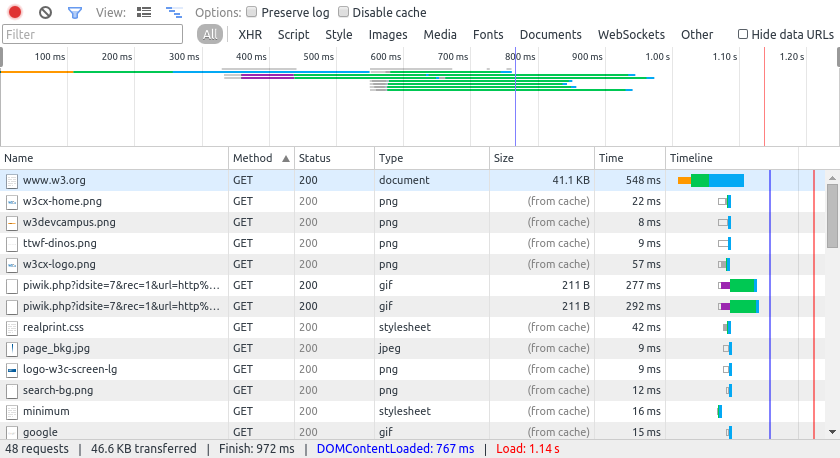
\includegraphics[width=\linewidth]{http_requests}
	\caption{Google Developer Tools window showing HTTP Requests\label{http_requests}}	
\end{figure}

In the above example only the GET HTTP method is used, because the client only requests data from the server, without
sending any data itself. If the client needs to send data to the server, such as form data, or a file, it would still
initiate the connection (the server cannot make requests, only respond, another consequence of statelessness), using
the POST method. While this approach is suitable for a passive, document-based web, where interaction is limited to
jumping from document to document, the web has quickly evolved into an application-based model, where full UIs take
place in the browser space, requiring data be constantly sent back and forth between client and server, in realtime.
This project is one such application.\\

The only way to do this with standard HTTP is periodic polling, which entails large server and network loads. Some
stopgap solutions exist to minimize this overhead, most relevant of which is the Comet web application model. Comet is
based on the concept of long-polling: effectively ``hanging'' the server response until the requested data is
available, and calling another request once the data is received. This approach  still causes increased server loads
but allows some semblance of real-time data transmission. The possibility to use only one connection, as seen in the
previous example was another improvement that became standard in HTTP 1.1. With the HTTP/2 Standard (published in May
2015), the server is allowed to effectively ``push'' data to clients by queuing up more responses than received
requests. However, none of these modifications and hacks are a complete, elegant solution to the problem, given that
HTTP was never intended to be a real-time protocol.\\

That is why other technologies have taken over this new realm of interactivity, providing much more than the ``big,
virtual documentation system in the sky'' \cite{bernerslee09} envisioned by Berners-Lee more than 25 years ago. Some
of them are key parts of this project, as the following sections describe. Still, HTTP remains the initiator for all
these other technologies to function. As of today, any web page you open, no matter how complex the code served in
javascript or flash or any other plug-in still begins with a simple GET request and response.
\section{HTML} \label{HTML}
HTML (Hypertext Markup Language) is the language in which web pages are written. It was created in 1989 by Tim
Berners-Lee as part of his WorldWideWeb, a set of documents linked between each other on a network using the Internet
protocol. It was initially based on SGML (Standard Generalized Markup Language) a document markup language released in
1986 as an ISO Standard (ISO 8879:1986 -- Information processing -- Text and office systems), which was itself derived
from GML (both an acronym for Generalized Markup Language and for Goldfarb, Mosher, Lorie, the last names of its
developers), developed by IBM in 1969.\\

Markup languages in general existed before digital media and still exist in paper based documentation (blue/red
annotations used by editors because lithography/photography/xerography did not capture these colors, the engineering
code for editing documents red = add, blue = delete, green = comment, and many others). In general, markup is a way to
add information regarding the document's structure, presentation, state of development, comments, author, date,
copyright, etc. in a way that is distinguishable from the content of the document. For digital media, it also needs to
be machine-readable, which simply means that a computer must be able to parse this data to extract information. There
are basically two ways of doing this:
\begin{enumerate}
	\item Procedural Markup: A source text is written with instructions for a processing program (equivalent to a
  compiler) to construct the final document. A good example of this method is \TeX, the typesetting system underlying
  the \LaTeX\ macro language (which is itself a mixture of procedural and declarative markup), used to write this
  document.
	\begin{figure}[ht]
    \subfloat[Procedural Source (\LaTeX)]{{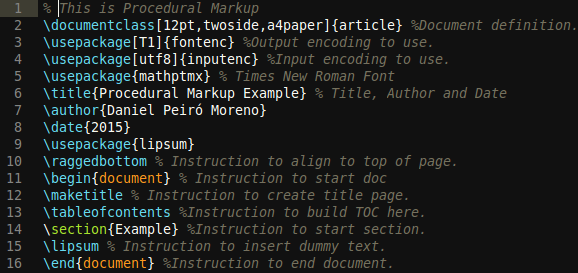
\includegraphics[width=\linewidth/2]{html_procedural_in}}}
    \subfloat[Procedural Output (PDF)]{{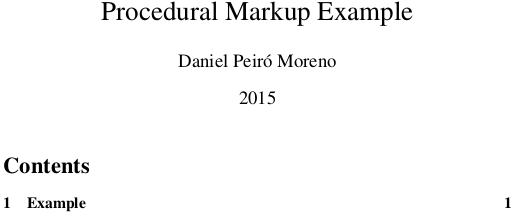
\includegraphics[width=\linewidth/2]{html_procedural_out}}}
    \caption{Procedural Markup Example}
	\end{figure}
	\item Declarative or Descriptive Markup: The content of the text is labeled or ``tagged'' with the markup, without
  giving any instructions on how to process these labels. HTML (especially before HTML5) and XML are clear examples of
  this method.
	\begin{figure}[ht]
    \subfloat[Declarative Input (HTML5)]{{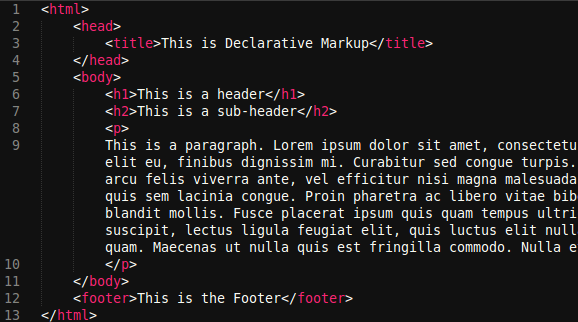
\includegraphics[width=\linewidth/2]{html_declarative_in}}}
    \subfloat[Declarative Output (Google Chrome)]{{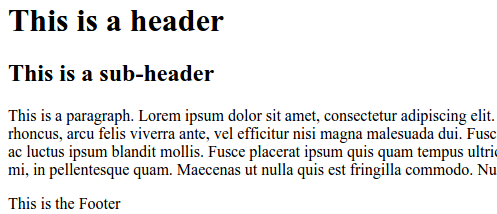
\includegraphics[width=\linewidth/2]{html_declarative_out}}}
    \caption{Declarative Markup Example}
	\end{figure}
\end{enumerate}
HTML and its precursor SGML are essentially declarative markup languages. The main advantage of declarative markup,
and more generally the declarative programming paradigm is the decoupling of the intended result and the processing
required to achieve it. This has been crucial for HTML to be able to evolve and adapt dynamically over decades of
technological innovation. The computers and programs used in 1989 have very little in common with those used today in
many cases. A markup language designed to be ubiquitous, read on an ever changing array of software and hardware
platforms and permanently backwards compatible, where a web page designed in 1991 is just as valid as one designed
using the last specification, has to be as procedurally oblivious as possible.\\

The basic HTML markup unit is the tag. A tag is simply a keyword surrounded by brackets. HTML tags usually come in
pairs, an opening tag and a closing tag (designated adding a forward slash after the first bracket), that give markup
information on the enclosed content:
\begin{figure}[h]
\centering
\RecustomVerbatimEnvironment{Verbatim}{BVerbatim}{}
\begin{minted}[breaklines,fontsize=\footnotesize]{html}
<!--This is a comment-->
<h1>This is a heading</h1>
<p>This is a paragraph</p>
<div>This is a section</div>
<table>
  <tr>
    <th>Table Header Cell 1</th>
    <th>Table Header Cell 2</th> 
  </tr>
  <tr>
    <td>Table Cell 1</td>
    <td>Table Cell 2</td> 
  </tr>
</table>
<ul>
  <li>List Element 1</li>
  <li>List Element 2</li>
  <li>List Element 3</li>
</ul>
<a href="http://www.w3.org">This text links to W3C Web Page</a>
\end{minted}
\caption{Declarative HTML Tags}
\end{figure}\\
All of the tags in the above example are purely declarative. They state what the enclosed text is, leaving it up to
the parser how to obtain the desired result. To extend markup within a tag, attributes are added and given a value. For 
example, the href attribute in the <a> hyper link tag above points to the URL the browser will go to when the text is 
clicked. As the web evolved since it's inception, adding interactivity to documents, more tags were added to HTML that 
weren't so clearly declarative and had a behavioral component, as well as semantic attributes:\\
\begin{figure}[h]
\centering
\RecustomVerbatimEnvironment{Verbatim}{BVerbatim}{}
\begin{minted}[breaklines,fontsize=\footnotesize]{html}
<form action="" method="">
  <input type="text" name="input1"><br>
  <input type="text" name="input2"><br>
  <input type="button" value="value0" onclick="">
  <input type="checkbox" name="input3" value="value1">
  <input type="radio" name="input4" value="value2"><br>
  <input type="radio" name="input5" value="value3">
  <input type="submit" value="Submit">
</form>
\end{minted}
\caption{Behavioral HTML Tags}
\end{figure}\\
These behavioral tags (and many others) were a response to the demand for a more interactive web, not only composed of
linked documents, but of applications implementing business logic and data transactions. They were added by web
browser developers independently, and in consequence were incompatible with other software as well as poorly
documented. In 1994, Tim Berners-Lee created the W3C (World Wide Web Consortium) to solve this problem, attempting to
achieve consensus between browser developers developing standard versions of HTML. This helped HTML remain relatively
simple and consistently usable across browsers. The W3C also attempted to standardize the way browsers parsed HTML,
which initially was very lenient to errors. The repercussions of these attempts will be discussed in section
\ref{HTML5}, specifically related to HTML5, as they indirectly led to the standard.\\

HTML tags can be nested, with the outer tags being called parent tags, and tags enclosed by others called children.
This nested structure, which can also be seen as a tree structure is called the Document Object Model or DOM for short.
This model represents all of the objects included in the document in nodes, with parent nodes encapsulating child nodes,
and one root node that encapsulates all of them. To create the DOM, different browsers use different methods, called
layout engines that parse the HTML to create the DOM Tree. This tree serves only the purpose of correctly representing
nested content on a page, where static web pages are concerned. However, the DOM is crucial for dynamic web pages, as it
provides external controllers, such as JavaScript a model to interact with (see section \ref{JavaScript} on JavaScript).\\

In this project there is just one HTML document (albeit one composed of more than 500 lines of markup) and therefore only
one DOM Tree, as it implements the ``Single Page Application'' user interface paradigm as a means to make the user
experience more fluid and similar to that of a native program. The structure of the page, which is decidedly non-
declarative as a whole, is nonetheless defined using almost exclusively declarative tags. Only multimedia is truly
generated dynamically on the page, with everything else being declared statically, with the caveat of being bi-
directionally bound to a model which in turn is dynamically changed (see section \ref{AngularJS} on AngularJS).\\

The declarative markup method has many advantages as shown: simplicity, portability, light-weight parsing... But it's
main flaw remains that it lacks the ability to create complex structures, interactive structures, and dynamic
structures. Declarative markup is distinctly static in nature: once parsed, the content is presented and remains the
way it was declared (at least in purely declarative tags). This is not a flaw inherent to its design, as it was designed
to markup documents, but one created through the evolution of the web. HTML as a language has itself evolved, blurring
the lines of declarative and behavioral markup (see section \ref{HTML5} on HTML5 for more), but for interactivity and
complexity to truly flourish, markup as a whole just isn't enough. As early as 1995, it became evident that the web
needed a programming language. That language was JavaScript.
\section{JavaScript} \label{JavaScript}
\begin{figure}[h]
\centering
\includesvg[width=1.1\linewidth/4]{./img/javascript}
\caption{JavaScript Badge}
\end{figure}
JavaScript is a programming language. The most common use for JavaScript is running scripts alongside web pages, making
them dynamic and interactive in ways HTML alone cannot. JavaScript was created by Netscape, an early web browser vendor
and developer in 1994, as part of its Netscape Navigator browser. Originally named Mocha, then LiveScript and finally
JavaScript (not because it is related to the Sun developed language, but as an attempt by its creators to use the
popularity of Java for marketing reasons). It was initially conceived as a ``glue'' programming language to be used by
web designers with little programming knowledge or experience to include Java (considered a more ``serious'' and powerful
language at the time) applets in their pages without necessarily knowing anything about Java programming. It quickly
evolved beyond that, becoming a programming language in it's own right. After Microsoft included it in Internet Explorer
3.0 in 1996 (as JScript, to add to the naming confusion), Netscape sought to standardize the language through the ECMA
standards organization, eventually leading to ECMAScript, the current technical name of the language (used only in
standard versions). The current standard is ECMAScript 5 originally released in 2009, while ECMAScript 6 will be released
sometime in 2015. Although JavaScript is mainly used client-side even today, it was originally conceived to also run
server-side. This concept was widely ignored during the early days of the web, focusing on client-side dynamic scripting,
while using other languages (PHP, CGI, Perl, etc.) on the server-side. The late 2000s and early 2010s have seen a
resurgence of the idea of server-side JavaScript allowing full-stack (front-end to back-end in javascript) applications,
like this project, to exist. This will be covered in section \ref{TheMEANStack} on the MEAN Stack.\\

The formal classification and description of JavaScript as a language is beyond the scope of this overview, so it won't
be discussed here. Suffice it to say that it's a prototype-based, dynamically-typed scripting language, which allows it
to implement multiple programming paradigms (imperative, functional and object oriented), sacrificing performance (as do
all dynamic languages) and formal elegance for a high level of abstraction, flexibility and dynamic execution.\\

The key aspect of client-side JavaScript is that runs in the browser, dynamically modifying the HTML document. A
JavaScript script is included in an HTML document simply by using the script tag:
\begin{figure}[h]
\centering
\RecustomVerbatimEnvironment{Verbatim}{BVerbatim}{}
\begin{minted}{html}
<script type="text/javascript" src="examplescript.js"></script>
\end{minted}
\end{figure}

As seen in section \ref{HTTP} on HTTP, this tag will trigger a HTTP GET request to the server for the text file
``examplescript.js'', that the browser will parse as JavaScript, and dynamically execute, with total transparency
from the users point of view. This script could, in a typical early web use-case, modify the web page dynamically,
without necessarily triggering new HTTP requests to the server, given that once the script is served, it is running
independently on the client system. For modifications to be possible, a machine-readable model of the web pages' content
and markup is required. The DOM (Document Object Model, see section \ref{HTML} on HTML) is the convention used to model
the page, and is kept in memory by the JavaScript Engine as the global ``state'' of the page. Scripts can then get
information from the model, as well as control and modify the model. The browser will then refresh the representation of
the page, following a classic Model (DOM), View (Browser window), Controller (JavaScript scripts) paradigm.\\

This use-case, while still the most extended use for JavaScript has given way in the last decade and a half to a much
more behavior-centric use, where JavaScript no longer is an add-on or enhancement to HTML, as much as a fundamental part
of how we understand web pages, to the point where the latest standard in HTML includes many tags that are simply useless
without JavaScript to provide the behavior behind them. This demand for interactivity has also led to some pages that are
sloppy when it comes to separating behavior and structure of a web application, tending to use JavaScript for everything,
even when HTMLs declarative approach is more appropriate for a given use-case, simply because JavaScript is more
``comfortable'' from a programmers perspective. This brings with it code maintainability, elegance and performance issues
if not handled correctly. To help maintain declarative and behavioral code separate, and use each one when appropriate,
JavaScript frameworks such as AngularJS have appeared, allowing highly dynamic, complex, single-page web applications to
keep a Model-View-Controller paradigm. This framework, as part of the MEAN Stack, is used in this project (see section
\ref{AngularJS} on AngularJS).

JavaScript essentially provides behavior, interactivity and dynamism to otherwise static HTML. Other methods of adding
these traits to web pages exist and some remain popular today. Java Applets run in a JVM (Java Virtual Machine) once
executed from an HTML document. Adobe Flash (previously Macromedia Shockwave Flash) allows full animations, video and
audio to play embedded inside of a web page. Microsoft Silverlight (now deprecated) served a similar purpose as Flash.
All of these technologies had the major flaw of not integrating with HTML as much as substituting it, or embedding a
``black-box'' in it. This impacts platform compatibility, performance, and accessibility (without going in to the
problems that arise from proprietary technologies). Of the previous, only Flash remains relevant today, mainly as a means
to provide multimedia content, where the HTML standard is considerably lagging behind. But even then, Flash today is
either incompatible or unsupported on all major mobile platforms, and is quickly being substituted with HTML5 by
multimedia providers (Youtube, for example, now defaults to an HTML5 player as opposed to Flash). JavaScript on the other
hand has been consistently relevant since it's inception and continues to grow in importance as a web technology,
expanding to the back-end, and becoming inextricably embedded in the latest HTML standards. This is precisely because it
doesn't try to substitute or deprecate HTML, but complements it by adding behavior to structure, while allowing both to
remain separate.
\section{CSS} \label{CSS}
\begin{figure}[h]
\centering
\includesvg[width=\linewidth/4]{./img/css3}
\caption{CSS3 Badge}
\end{figure}
HTML provides structure to web documents. JavaScript adds behavior, turning documents into applications. CSS (Cascading
Style Sheets) adds style, giving the document renderer instructions on the presentation of the structure created with HTML.
This gives documents and applications, which have no inherent visual representation, a distinct style, as chosen by the
designer, not by the renderer. CSS was created by Håkon Wium Lie and Bert Bos in 1994. It was originally named Cascading
HTML Style Sheets (CHSS), as it was aimed exclusively at HTML styling. The H was soon dropped from the name, as the authors
wanted CSS to be applicable to other markup languages. CSS, like HTML wasn't the first language of it's kind. Style sheet
languages like DSSSL (Document Style Semantics and Specification Language) or FOSI (Formatted Output Specification
Instance) were created for HTMLs precursor, SGML (see section \ref{HTML}). However, these languages didn't allow for style
sheets to be separated from the document, and were therefore unsuitable for the nature of the web, while also being deemed
too complex. CSS has been standardized by the W3C since it's creation, producing three main recommendations:
CSS1 in 1996, CSS2 in 1998, and CSS3 which was divided into modules for different aspects of the language, some of which
have already been finished in the last few years, others still evolving. CSS4 development has begun on completed modules,
but will not be extensively worked on until CSS3 is finalized.\\

Before CSS, HTML either was devoid of any presentational specifications (leaving all styling to the default specified by
the renderer, making all web pages quite simple and unappealing) or had to be styled from within HTML. This was done using
presentational tags, which remained part of HTML standard until HTML4 (see figure \ref{presentational_tags}).\\
\begin{figure}[h]
\centering
\RecustomVerbatimEnvironment{Verbatim}{BVerbatim}{}
\begin{minted}{html}
<h1>
  <font size="3" color="red">This is a heading</font>
</h1>
<body background="bgimage.jpg"><!--Use image as background-->
<strike>This text is strikethrough.</strike>
<img src="exampleimage.png" border="5"><!--Image with 5px border-->
<center>This text will be center-aligned.</center>
</body>
\end{minted}
\caption{Deprecated Presentational Tags \label{presentational_tags}}
\end{figure}

This presented the problem of mixing declarative, structural markup with styling, making the structure much less clear to
the editor, which in turn led to error-prone design, while still being a limited solution, since the amount of tags needed
to be kept in check, if there was to be any structure to the language.\\

CSS allows, similarly to how JavaScript does with behavioral components, the addition of style without substituting
structure while keeping a separate environment for each. With CSS, the only tag necessary is the script tag, or if included
from another file, the link tag:
\begin{figure}[h]
\centering
\RecustomVerbatimEnvironment{Verbatim}{BVerbatim}{}
\begin{minted}{html}
<head>
<link rel="stylesheet" type="text/css" href="stylesheet.css">
</head>

<!--OR-->

<style>
h1 {
font-size: 3px;
color:red;
}
</style>
\end{minted}
\caption{Linking or including CSS in HTML}
\end{figure}
This separates the structure and the presentation of the web page neatly, allowing both to remain clear, readable and
maintainable.\\

The main styling unit of CSS is the rule. A rule is composed of selector and a declaration block. A selector specifies the
target of a set of style specifications (declarations) that follow in the declaration block. In the previous example, there
is only one rule, with selector h1 and declarations font-size and color. This rule will target all h1 tags present in the
document and apply the declarations inside the declaration block to the content of the tag. There are a wide range of
selectors available, from the simplest like the wild-card, *, that targets all elements, to complex, composite selectors
that target elements with certain attribute values (particularly useful is the ".class" selector that targets all elements
with a certain class attribute value), pseudo-selectors that target elements under certain circumstances (``:hover''
targets elements with the mouse over them), etc. which allow complete control over the presentation of web pages.\\

While rules provide granular presentational control over the web page, as a standalone, they would be cumbersome at best
and impossible to implement at worst were it not for cascading. Cascading allows the definition of a hierarchical structure
in the way rules are applied, where rules with a higher priority overwrites lower priority rules. There are several
priority definitions (for example, in line style tags prevail over included stylesheets), but the most important is
selector specificity. If an element fits the target for two or more selectors, the one with the highest specificity will
prevail, if that rule defines a conflicting declaration. For example:
\begin{figure}[h]
\centering
\RecustomVerbatimEnvironment{Verbatim}{BVerbatim}{}
\begin{minted}{css}
/* Applies to all elements */
* {
  color: green;
  text-align: center;
}

/*
  Applies to h1 elements.
  Overrides color from *,
  keeping text-align: center.
*/
h1 {
font-size: 3px;
color:red;
}

/*
  Applies to p elements nested in div elements.
  Overrides both * declarations.
*/
div > p {
  color: blue;
  text-align: right;
}

/*
  All other elements will apply *,
  without need for more rules.
*/
\end{minted}
\caption{Cascading CSS Specificity.}
\end{figure}
\\(Note: Use of * selector is somewhat inefficient and inelegant, used here for illustration purposes).\\

Without this feature, it would be necessary to specify styles for each type of element, or leave some up to the renderer.
This, as previously stated would be tedious for document based pages, and near impossible for applications.\\

This project implements the ``Single Page Application'' user interface pattern, and therefore only one style sheet is used.
In websites with multiple web pages, there's normally one root style sheet that defines the general presentation of the
site, common to all pages, and each page may have it's own particular style sheet for more specific presentation
specification. This allows for neat compartmentalization of styling, which benefits maintainability, future development and
documentation.\\

Some of the more modern modules of CSS3 used in this project (media queries and transitions) will be discussed in section
\ref{HTML5} on HTML5. Even though CSS3 is technically a separate entity and W3C standard, it is most certainly part of the
wider definition of HTML5 as "the cornerstone for modern web applications"\cite{w3c11}.
\section{HTML5} \label{HTML5}
\begin{figure}[h]
\centering
\includesvg[width=1.4\linewidth/4]{./img/html5}
\caption{HTML5 Badge}
\end{figure}
HTML5 is the latest version of the HTML (see \ref{HTML} on HTML in general) Specification Recommendation developed and
published by the W3C (in its final form, development started outside the Consortium) released the 28th of October, 2014.
The significance of this date is somewhat diminished given that HTML5 has been in development since 2004, and many of the
APIs (Application Programming Interface) it specifies have been implemented in browsers preceding the formal release date,
in many cases years in advance.\\

The fundamental change between HTML5 and previous versions of HTML is the shift to a Web Application model from the
original Web Document model. This change came as a response to the direction the W3C had taken after the publication of
HTML 4.0 in 1997, which was much more conservative. At that time, the W3C was very concerned with broken HTML: it is
assumed (including by the W3C\cite{w3cwebquality02}) that 99\% of web pages are not valid HTML. This is made possible by
the lenient error handling methods used by browser HTML parsers. When a browser finds an error in an HTML document 
(incorrect tag spelling, unclosed tags, missing brackets, incorrect nesting order etc.), instead of stopping and not 
rendering the page, it works around the error, displaying the page as well as it can. This allows for web pages to have 
minor errors that do not alter the overall display of the page, remaining usable for most users, and more importantly, 
allowing anybody that has a basic knowledge of the language to write a web page without having to become an expert, 
effectively making HTML a much more accessible and universal language. The downside to this is inconsistency, which is 
what concerned the W3C: What methods are used in this lenient error handling? Are they to be standard? Proprietary? Which 
errors are permissible? Are future browsers going to be able to read invalid pages which were parsed with undocumented 
error handling methods? All these valid concerns lead the W3C to a drastic decision: draconian error handling.\\


The W3C established that the next HTML standard, called XHTML 1.0, would have to be well-formed XML (eXstensible Markup
Language, a profile of SGML) to be rendered. This, technicalities aside, meant that all documents that wanted to be valid
markup under the new specification, would need to have no errors for browsers to render them. If not, the page would not
render and an error message would be presented to the user. Even for a single mistyped tag. This also rendered all
previous, error laden web pages obsolete in the eyes of the W3C.\\

As discussed in previous sections, attempts to deprecate existing HTML or substitute it with something new, have been in
general unsuccessful. XHTML was no exception. Given that the benefits of upgrading were few, and barely apparent for the
general public, web creators didn't make the jump from HTML 4.0. XHTML 1.0 allowed, through a transitional loophole, the
possibility of declaring the document as XHTML while keeping lenient error handling from HTML 4.0. Even then, adoption was
slow, but when XHTML 1.1 closed this loophole, it sealed its fate as a failed ``upgrade''.\\

After XHTML, the W3C was at an impasse of sorts. It had spent years on the development of XHTML, which had a very low
adoption rate and the power of home computing was sky rocketing, leading to demands for web applications instead of
documents to increase immensely. In 2004, it held a workshop (The W3C Workshop on Web Applications and Compound Documents
\cite{w3c04}) to define the future of web applications. Many manufacturers and interest groups proposed that a series of
mid-level APIs should be developed as extensions to HTML and CSS for use in Web Applications as opposed to fully fledged OS
-Level APIs. This meant leaning toward in-browser solutions as opposed to ``black-box'' plug-in software (such as Java
Applets or Flash). This proposal was rejected (see Workshop Summary straw poll topic no. 3 in \cite{w3c04}), and led to a
group of the proposers to create a work group outside the W3C, the WHAT Working Group (Web Hypertext Applications
Technology Working Group). This group went in the opposite direction the W3C did to solve HTMLs error handling problems
and the evolution of the web. Instead of dropping error handling altogether, like XHTML did, the WHAT group decided it
would specify and document the way lenient error handling works, so that it would no longer rely on proprietary, poorly
documented solutions that made future proofing and maintaining compatibility among different browsers virtually
impossible. This wasn't as easy as the XHTML solution, in fact it took 5 years to complete, but it allowed full backwards
compatibility for older pages, a crucial aspect of evolving the web, as seen in previous sections. For Web Applications,
the WHAT group turned away from plug-ins, and started work on three of the most important multimedia APIs present in
HTML5: Canvas (direct-mode drawing) and native Audio/Video support.\\

In 2006, Tim Berners-Lee announced that the W3C would start working with the WHAT WG to evolve the web. The new HTML
Specification that would come from this new group, would be called HTML5.\\

HTML5 introduced a long list of new features to HTML, most of them directed at Web Application Development:
\begin{itemize}
  \item \textbf{Canvas Element}: Direct Mode 2D Drawing. Essentially allowing for fully native animations.
  \item \textbf{Audio and Video Element}: Native multimedia support, effectively deprecating flash.
  \item \textbf{Geolocation}: Allows sharing the clients location with the application seamlessly.
  \item \textbf{Local Storage}: Allows the application to store data on the clients computer.
  \item \textbf{Offline Web Applications}: Once downloaded, the application can run without being connected to the Internet.
  \item \textbf{WebSockets}: Full duplex communication between client and server, in one TCP connection. (Now a separate specification)
  \item \textbf{Web Workers}: JavaScript running in the background, taking full advantage of the client CPUs power for heavy tasks.
\end{itemize}
While others were much needed upgrades and deprecations of HTML 4.0 features, such as the addition of a wealth of new
controls to forms and semantic tags, as well as the removal of presentational tags altogether. Only the features used in
this project will be discussed briefly further.
\subsection{HTML5 Semantics}
\begin{figure}[h]
\centering
\includesvg[width=1.4\linewidth/8]{./img/html5_semantics}
\caption{HTML5 Semantics Badge}
\end{figure}
HTML5 Semantics are used to more clearly and succinctly define the elements content. This improves the readability of the
markup and allows browsers to make better accessibility tools. It makes the markup easier to read by eliminating
unnecessary text:\\

\begin{figure}[h]
\centering
\RecustomVerbatimEnvironment{Verbatim}{BVerbatim}{}
\begin{minted}{html}
<!--In XHTML 1.0-->
<!DOCTYPE html
          PUBLIC "-//W3C//DTD XHTML 1.0 Strict//EN"
          "http://www.w3.org/TR/xhtml1/DTD/xhtml1-strict.dtd">
<html xmlns="http://www.w3.org/1999/xhtml"
      lang="en"
      xml:lang="en">
</html>
<!--In HTML5-->
<!DOCTYPE html>
<html></html>
\end{minted}
\caption{HTML5 Semantics: Text Usage Comparison}
\end{figure}
And by giving names to typical web page components:\\

\begin{figure}[h]
\begin{center}
  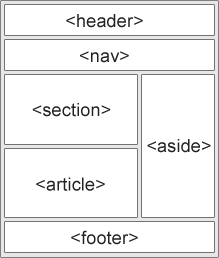
\includegraphics[width=\linewidth/3]{html5_layout}
  \end{center}
  \caption{HTML5 Semantics: Typical Page Layout. Source: \href{http://www.w3schools.com/html/html5_semantic_elements.asp}{
  W3Schools}.}
\end{figure}
This allows web browsers to better understand what the content is declared as, and choose to present it in different ways (
for example, a page with an article and a header might be presented differently on a mobile browser to enhance the reading 
experience), and allows for accessibility features such as text-to-speech to present the content in a fitting manner.\\

In this project, the page is written using HTML5 semantics, reducing the amount of superfluous text, making it easier to
read (taking into account the complexity of the liquid layout). It also uses the header and footer tags to frame the
controls, using the header as the title of the page, and the footer to include copyright acknowledgments and references.
\begin{figure}[h]
\begin{center}
  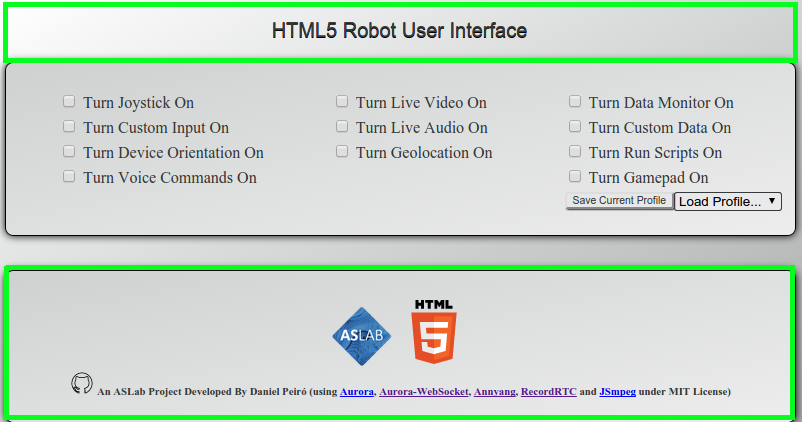
\includegraphics[width=\linewidth]{html5_headerfooter}
  \end{center}
  \caption{HTML5 Semantics: Use of Header and Footer (Marked in green) in HRUI}
\end{figure}
\subsection{HTML5 Canvas Element}
\begin{figure}[h]
\centering
\includesvg[width=1.4\linewidth/8]{./img/html5_canvas}
\caption{HTML5 Graphics Badge}
\end{figure}
The Canvas element is, in the simplest terms possible, a rectangle in a web page in which a JavaScript script can draw
anything. It allows things as simple as drawing a line with the cursor, to full fledged game graphics, and requires
nothing but a canvas element (\mintinline{html}{<canvas></canvas>}) and access from JavaScript to said element. By
changing the drawing at a fast enough frequency, animation becomes trivial.\\

In this project, the canvas element is used for three of its modules. It's used to create virtual joysticks for the user
to control dynamically with the mouse or using a touch interface (see section \ref{joystick} on the Joystick input module).\\

\begin{figure}[h]
\begin{center}
  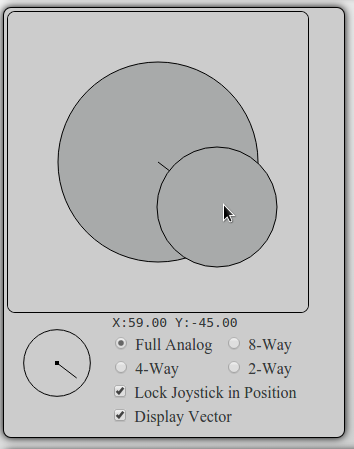
\includegraphics[width=\linewidth/3]{joystick}
  \end{center}
  \caption{HTML5 Canvas: Joystick in HRUI. (2 Canvas Elements: Joystick and Vector)}
\end{figure}
It's used for the live video feed, using JSMpeg, a MPEG1 decoder written in JavaScript (see section \ref{livevideo} on the
Live Video module). It's also used for the dynamic obstacle map in the data monitor module (see section \ref{datamonitor}),
which can be generated from the server, uploaded by the user or can even be drawn on the fly with the cursor or touch
interfaces (see figure \ref{html5_map}).\\

\begin{figure}[h]
\begin{center}
  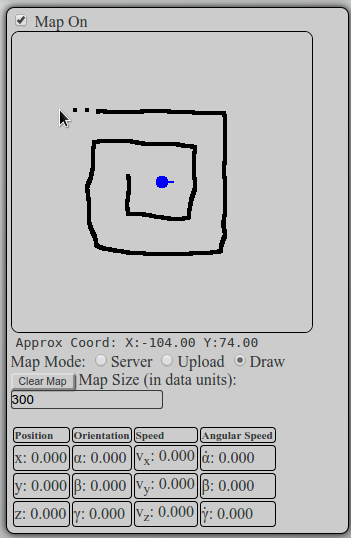
\includegraphics[width=\linewidth/3]{html5_map}
  \end{center}
  \caption{HTML5 Canvas: Map in HRUI. (Black: Drawn Obstacles. Blue: Robot Pos.)\label{html5_map}}
\end{figure}
The Canvas API allows for essentially any sort of content to appear on a website natively without the need for flash, which
was the go-to resource for animation previously. This amounts to a big leap in graphics and animation versatility for HTML.\\

\subsection{HTML5 WebSockets}
\begin{figure}[h]
\centering
\includesvg[width=1.4\linewidth/8]{./img/html5_connectivity}
\caption{HTML5 Connectivity Badge}
\end{figure}
WebSockets allow for full-duplex communication between server and client using one TCP connection. As its name implies it's
most easily described as an implementation of TCP/IP Sockets for the web. It allows for fully bidirectional communication,
using only one HTTP request (see section \ref{HTTP} on HTTP), that is upgraded to a WebSocket connection. This HTTP handshake
is important, as it allows for a graceful backwards compatibility, using the same technology as standard web pages.\\

WebSockets are essential for this project. As a real-time application, data needs to move to and from the client and the
server constantly to relay instructions from the controls to the back-end, an update output data to the front-end.
Furthermore, to live stream media from the server to clients, WebSockets are used, providing minimal latency. Without
WebSockets this project would be almost impossible to achieve, with any measure of success.\\

The WebSockets API in HRUI is implemented in two forms: raw and through the Socket.IO framework. The raw form creates and uses
WebSockets through direct calls to the API and is used for media streaming. The Socket.IO framework adds a layer of
abstraction to WebSockets, by creating an event-based model. An event is a message that is broadcast by an emitter and
captured by a listener. The emitter and listener are the server and client, and vice versa. An event carries attached to it a
JavaScript object which will be received by the listener. The programmer creates these asynchronous events on either the
server or the client, establishing the behavior of the listener. For example: Every 50 ms the back-end wants to send the front-
end an update on the value of X in the robots position. With Socket.IO (after setup) the code would be:\\

\begin{figure}[h]
\centering
\RecustomVerbatimEnvironment{Verbatim}{BVerbatim}{}
\begin{minted}[fontsize=\footnotesize]{javascript}
//On the Server side:
//[...](setup and surrounding code omitted for clarity)
var x = 10; //value of robot X coordinate (defined here for brevity)

socket.emit("UPDATE_X", x);
//emit an event with message UPDATE_X and data x (value: 10)

//On the Client side:
//[...](setup and surrounding code omitted for clarity)
socket.on("UPDATE_X", function(received_x) {
              console.log(received_x);
            };
//listen for an event with message UPDATE_X
//and print the value of the data received to the console.
\end{minted}
\caption{HTML5 WebSockets: Socket.IO Event Example}
\end{figure}
This added layer of abstraction makes using WebSockets very simple, needing only to define when and where in the code events
are generated and adding listeners for these events. It also makes code much easier to understand, and much more structured,
closer to the business logic and separated from low level serializing and underlying connections.
\subsection{HTML5 Device Access}
\begin{figure}[h]
\centering
\includesvg[width=1.4\linewidth/8]{./img/html5_device_access}
\caption{HTML5 Device Access Badge}
\end{figure}
HTML5 Device Access allows the web application to use the hardware of the machine the browser is running on. This means
anything from microphones and cameras to accelerometers and GPS data.\\

HRUI makes full use of three of these APIs:\\

\begin{itemize}
  \item \textbf{Microphone}: The Voice Command module (see section \ref{voicecommands}) uses device access to receive audio
  from the users microphone, which is then recognized (using Annyang) into commands which are sent to the server for use (see
  figure \ref{html5_voice}). It also uses the WebRTC API to enable an alternative in non-chromium browsers that don't have the
  speech recognition API, by recording a 5 second audio clip that is sent as a .wav file to the server. WebRTC started out as
  part of HTML5 but has spun out into its own specification, that allows for peer-to-peer server-less audio and video sharing,
  among many other multimedia uses which are outside of this reports scope, since they're not used in this project.

  \begin{figure}[h]
    \begin{center}
      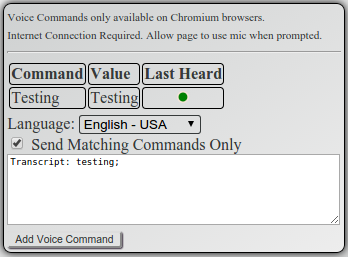
\includegraphics[width=\linewidth/2]{html5_voice}
    \end{center}
    \caption{HTML5 Device Access: Voice Commands in HRUI.\label{html5_voice}}
  \end{figure}
  \item \textbf{Device Orientation}: The Device Orientation module (see section \ref{deviceorientation}) gets the orientation,
   velocity and acceleration from the device (if available) and sends it to the server for use (see figure 

  \ref{html5_orientation})
  \begin{figure}[h]
    \begin{center}
      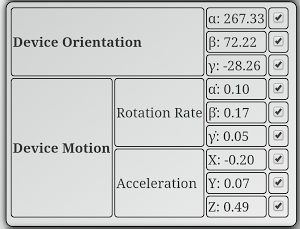
\includegraphics[width=\linewidth/2]{html5_orientation}
    \end{center}
    \caption{HTML5 Device Access: Device Orientation in HRUI.\label{html5_orientation}}
  \end{figure}
  \item \textbf{Gamepad}: The Gamepad module (see section \ref{gamepad}) uses the Gamepad API to get the inputs of a gamepad
  connected to the client machine and send them to the server for use. This extends the HRUI web application controls to
  virtually any device that can be connected to a web capable device as an input, allowing for external hardware to function
  seamlessly with this project with little to no integration effort. However, this API is still experimental at the time of
  writing, and support is limited to a few browsers (Chrome and Firefox mainly), with different implementations that require
  tweaking of parameters (mainly the mapping of buttons, which changes from Chrome to Firefox and with the controller in use)
  for consistent usage.
\end{itemize}
\subsection{HTML5 Styling}
\begin{figure}[h]
\centering
\includesvg[width=1.4\linewidth/8]{./img/html5_css3}
\caption{HTML5 Styling Badge}
\end{figure}
HTML5 Styling is actually a misnomer, albeit one used by the W3C, because it considers that HTML5 refers to more than just the latest HTML Recommendation, encompassing several specifications and should be used as an umbrella term to encapsulate all technologies of the modern web, calling HTML5 "The cornerstone for modern Web applications"\cite{w3c11}. This is cause of some debate among enthusiasts, but controversy aside, the fact is that HTML5 has no significant styling features (in consonance with the separation between declarative and presentational discussed in previous sections), relying on the CSS3 (Cascading Style Sheets, see section \ref{CSS}) specification for innovation in this aspect.\\

In HRUI many new CSS3 features are used to make the application more visually attractive and useful on different devices:\\

\begin{itemize}
  \item \textbf{Media Queries}: One the most useful additions made to CSS3 is the ability to apply styles to different viewports (the space where the web page is rendered in a browser) and device types without having to make different versions of the site, by using media queries. A media query basically defines a subset of styling rules that apply only to viewports that fit a certain criteria, while keeping in place the cascading nature of CSS. This means that by making, for example, a media query on the pixel width of the screen, a set of rules will be applied that can drastically change the presentation of the page. In HRUI only one media query is made, specifically to target smartphones (truncated for brevity):\\

  \begin{figure}[h]
    \centering
    \RecustomVerbatimEnvironment{Verbatim}{BVerbatim}{}
    \begin{minted}[fontsize=\footnotesize]{css}
      @media only screen and (max-width: 480px) {
          .frame {
              width: 100%;
          }
          #rightColumn, #centerColumn, #leftColumn {
              float: left;
              clear: both;
              width: 98%;
          }
      }
    \end{minted}
    \caption{HTML5 Styling (CSS3): Media Query in HRUI}
  \end{figure}
  Which targets screens under 480 pixels wide and applies the enclosed rules only to those screens. All other styling is maintained and applied, through cascading. These rule (and others omitted for brevity) make all modules occupy the whole width of the screen, more appropriate for small, touch based devices than the three-column default for computers and tablets. The user can then scroll through the modules to use them since including more than one module on a smartphone screen at once would clutter the interface and make it virtually unusable. This approach makes a necessary compromise by allowing the active visualization of one module at a time, while allowing all modules to run in the background, visible at the slide of a finger.
  \begin{figure}[h]
  \captionsetup{justification=centering}
      \begin{center}
        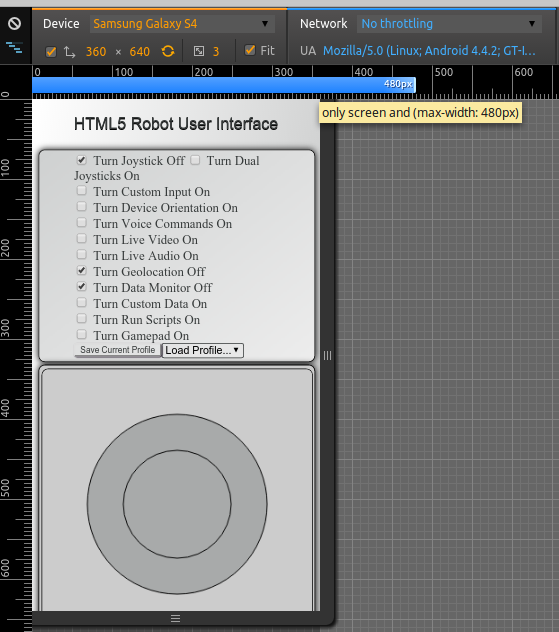
\includegraphics[width=\linewidth/3]{html5_css_mq2}
      \end{center}
      \caption{HTML5 Styling (CSS3): HRUI Smartphone version\\(simulated SGS4 using Chrome Dev Tools. Blue bar marks the detected media query)}
  \end{figure}
  \begin{figure}[h]
    \begin{center}
      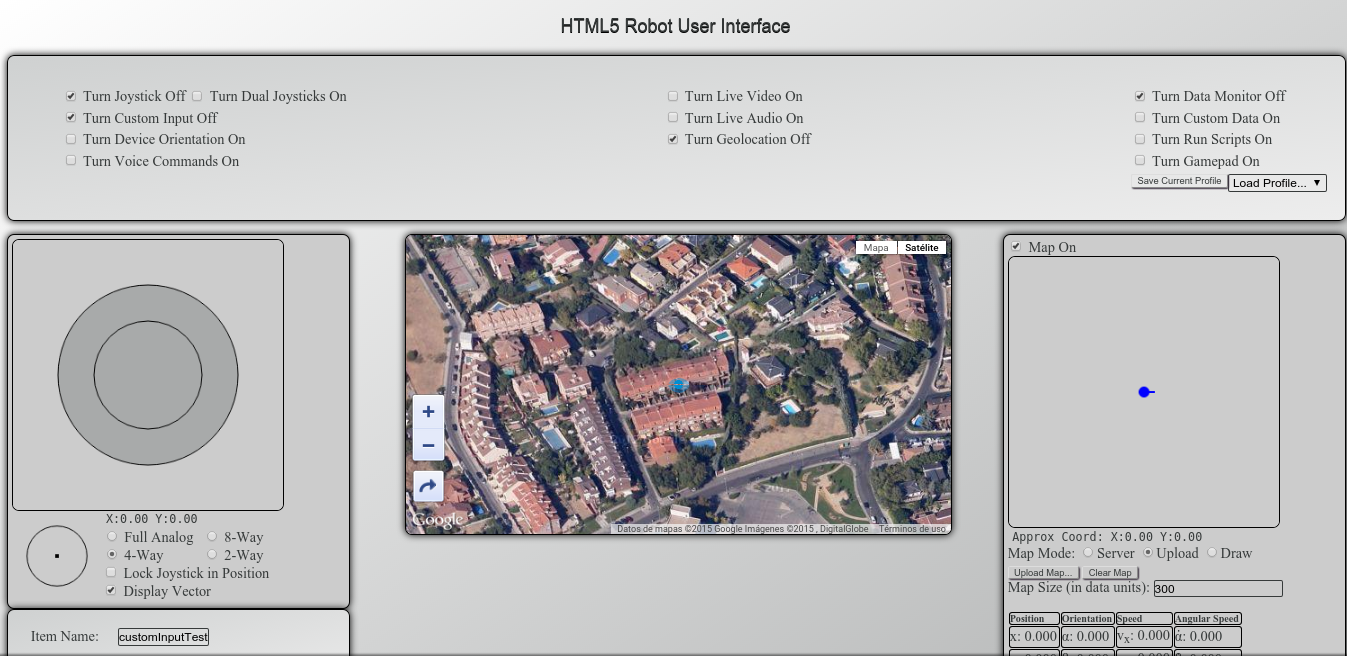
\includegraphics[width=\linewidth/2]{html5_css_mq1}
    \end{center}
    \caption{HTML5 Styling (CSS3): HRUI Laptop version}
  \end{figure}
  \item \textbf{Transitions}: CSS3 Transitions can make the value of element properties change over time, creating an attractive visual effect. HRUI uses this feature (combined with AngularJS Animate, see section \ref{AngularJS}) to animate module activation and deactivation with a fade in/out effect. Because this specification is still not final, it's still necessary to include vendor prefixes to transition rules, as each one implements the feature in slightly different ways.
  \begin{figure}[h]
    \centering
    \RecustomVerbatimEnvironment{Verbatim}{BVerbatim}{}
    \begin{minted}[fontsize=\footnotesize]{css}
    -webkit-transition: all 0.7s ease-in-out;
    -moz-transition: all 0.7s ease-in-out;
    -ms-transition: all 0.7s ease-in-out;
    -o-transition: all 0.7s ease-in-out;
    transition: all 0.7s ease-in-out;
    \end{minted}
    \caption{HTML5 Styling (CSS3): Transitions in HRUI.}
  \end{figure}
  \item \textbf{Gradients}: CSS3 Gradients make backgrounds change from one color to another across the surface of the element. It's used in HRUI to provide a smooth silver background with a lighting effect. As with CSS3 Transitions, vendor prefixes are required.
  \begin{figure}[h]
    \centering
    \RecustomVerbatimEnvironment{Verbatim}{BVerbatim}{}
    \begin{minted}[fontsize=\footnotesize]{css}
    background-image: -webkit-gradient( linear, left top, right bottom,...);
    background-image: -o-linear-gradient(right bottom, #CFD1D1 0%, #EDEDED 100%);
    background-image: -moz-linear-gradient(right bottom, #CFD1D1 0%, #EDEDED 100%);
    background-image: -webkit-linear-gradient(right bottom, #CFD1D1 0%, #EDEDED 100%);
    background-image: -ms-linear-gradient(right bottom, #CFD1D1 0%, #EDEDED 100%);
    background-image: linear-gradient(to right bottom, #CFD1D1 0%, #EDEDED 100%);
    \end{minted}
    \caption{HTML5 Styling (CSS3): Gradients in HRUI.}
  \end{figure}
  \begin{figure}[h]
    \begin{center}
      \frame{
\includegraphics[width=\linewidth]{html5_css_gradient}}
    \end{center}
    \caption{HTML5 Styling (CSS3): HRUI Header Gradient}
  \end{figure}
  \item \textbf{Pseudo Classes}: CSS3 Pseudo Classes are classes that target elements that match a given criteria. For example the :hover pseudo class targets elements over which the cursor is currently held. This allows for some dynamic style changes following user actions. Pseudo Classes existed in CSS2, but CSS3 added 16 new ones, including the one used in HRUI to change the color of disabled buttons to show the situation to the user.
  \begin{figure}[h]
    \centering
    \RecustomVerbatimEnvironment{Verbatim}{BVerbatim}{}
    \begin{minted}[fontsize=\footnotesize]{css}
    button:disabled {
    color: grey;
    box-shadow: inset 1px 1px 1px #3D3242;
    }
    \end{minted}
    \caption{HTML5 Styling (CSS3): Pseudo Classes in HRUI.}
  \end{figure}
  \item \textbf{Rounded Borders \& Box Shadows}
  \begin{figure}[H]
    \begin{center}
      \frame{
\includegraphics[width=\linewidth/4]{html5_css_round}}
    \end{center}
    \caption{HTML5 Styling (CSS3): HRUI Rounded Borders and Box Shadow}
  \end{figure}
\end{itemize}

\section{The MEAN Stack} \label{TheMEANStack}
\subsection{NodeJS}
\subsection{Express}
\subsection{MongoDB}
\subsection{AngularJS} \label{AngularJS}
\section{Python}
\section{Development Environment \& Tools}
\subsection{Linux}
\subsection{Sublime Text}
\subsection{Git}
\subsection{\LaTeX}
\subsection{PM2}
\section{Hardware}
\subsection{Khepera III}
\subsection{Crazyflie 2}
\subsection{Raspberry Pi 2}
